\section{Đề ôn thi giữa kỳ 2 toán 10}
\subsection{Phần trắc nghiệm}
Câu trắc nghiệm nhiều phương án lựa chọn. Học sinh trả lời từ
câu 1 đến câu 12. Mỗi câu hỏi học sinh \textit{chỉ chọn một} phương án.

\Opensolutionfile{ans}[Ans/Dapan]
 
\hienthiloigiaiex
%%%=============EX_1=============%%%
\begin{ex}%[0D3N1-5]%[Dự án đề kiểm tra Toán khối 10 GHKII NH23-24-Dot 2- Nguyen Chin Em]%[Deso9 - KNTT]
\immini{
Cho hàm số $y=f(x)$ có tập xác định là $[-3;3]$ và có đồ thị được biểu diễn bởi hình bên.
Mệnh đề nào sau đây là \textbf{SAI}?
\choice
{Hàm số đồng biến trên $(1 ; 3)$}
{Hàm số nghịch biến trên khoảng $(-1;1)$}
{\True Tập giá trị của hàm số là $[-3;3]$}
{Tập giá trị của hàm số là $[-1 ; 4]$}}
{
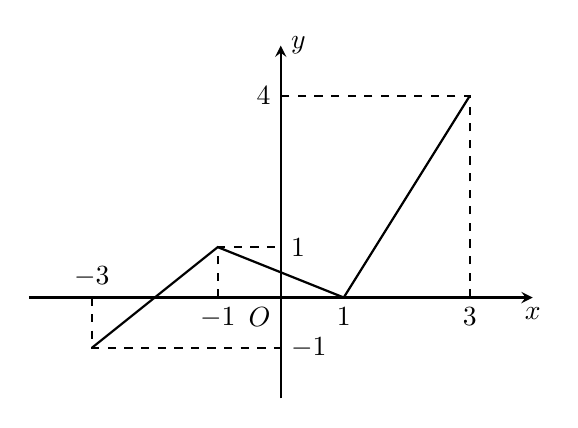
\begin{tikzpicture}[>=stealth, scale=.8,samples=200,xscale=1,yscale=.8,line width=.8pt]
   \draw[->,thick] (-4,0)--(4,0) node[below] {$x$};
 \draw[->,thick] (0,-2)--(0,5)node[right] {$y$};
 \draw (0,0) node [below left]{$O$};
\draw[dashed](-3,0)node[above]{$-3$}|-(0,-1)node[right]{$-1$} (-1,0)node[below]{$-1$}|-(0,1)node[right]{$1$} (3,0)node[below]{$3$}|-(0,4)node[left]{$4$} (1,0)node[below]{$1$};
\draw(-3,-1)--(-1,1)--(1,0)--(3,4);
\end{tikzpicture}
}
\loigiai{
Dựa vào đồ thị tập giá trị của hàm số $[-1;4]$, nên C sai.
}
\end{ex}
\begin{ex}%[0D3N2-3]%[Dự án đề kiểm tra Toán khối 10 GHKII NH23-24-Dot 2- Nguyen Chin Em]%[Deso9 - KNTT]
Cho hàm số bậc hai $y=a x^2+b x+c$ có giá trị lớn nhất là $10$ đạt được khi $x=2$ và đồ thị hàm số đi qua điểm $A(0 ; 6)$. Tổng giá trị $a+2 b$ là
\choice
{\True $7$ }
{$8$ }
{$9$ }
{$10$ }
\loigiai{
Do đồ thị đi qua $A(0 ; 6)$ nên $c=6$.\\
Vì Parabol có giá trị lớn nhất là $10$ có được khi $x=2$ nên
$\heva{&-\dfrac{b}{2 a}=2 \\&4 a+2 b+c=10}$.\\
Từ đó ta tính được $a=-1, b=4$ thoả mãn $a$ âm để có giá trị lớn nhất. Vậy $a+2b=7$.}
\end{ex}
\begin{ex}%[0D3H2-3]%[Dự án đề kiểm tra Toán khối 10 GHKII NH23-24-Dot 2- Nguyen Chin Em]%[Deso9 - KNTT]
Cho hàm số $y=ax^2+bx+c(a>0)$. Khẳng định nào sau đây \textbf{SAI}?
\choice
{Đồ thị của hàm số có trục đối xứng là đường thẳng $x=-\dfrac{b}{2 a}$}
{\True Đồ thị của hàm số luôn cắt trục hoành tại hai điểm phân biệt}
{Hàm số đồng biến trên khoảng $\left(-\dfrac{b}{2 a};+\infty\right)$}
{Hàm số nghịch biến trên khoảng $\left(-\infty ;-\dfrac{b}{2 a}\right)$}
\loigiai
{
Phương trình $ax^2+bx+c=0$, chưa khẳng định được có nghiệm, hay vô nghiệm. 
}
\end{ex}
\begin{ex}%[0D7N2-1]%[Dự án đề kiểm tra Toán khối 10 GHKII NH23-24-Dot 2- Nguyen Chin Em]%[Deso9 - KNTT]
\immini{
Cho hàm số $y=a x^2+b x+c$ có đồ thị như hình bên. Khẳng định nào sau đây là \textbf{đúng}?
\choice
{\True $a>0, b<0, c<0$}
{$a>0, b<0, c>0$}
{$a>0, b>0, c>0$}
{$a<0, b<0, c<0$}
}{
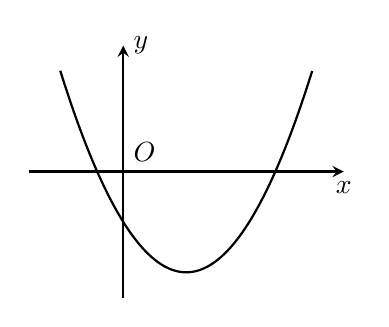
\begin{tikzpicture}[>=stealth, scale=.8,samples=200,xscale=1,yscale=.8,line width=.8pt]
   \draw[->,thick] (-1.5,0)--(3.5,0) node[below] {$x$};
 \draw[->,thick] (0,-2.5)--(0,2.5)node[right] {$y$};
 \draw (0,0) node [above right]{$O$};
\def\f(#1){(#1)^2-2*(#1)-1}
\draw[domain=-1:3,smooth,variable=\x,thick]plot (\x,{\f(\x)});
\end{tikzpicture}
}
\loigiai{
Dựa vào đồ thị ta thấy $a>0$, đồ th hàm số cắt trục ho tại 2 điểm, nên phương trình $a x^2+b x+c=0$ có 2 nghiệm, nên $c<0$. Chọn A.
}
\end{ex}
\begin{ex}%[0D7H2-6]%[Dự án đề kiểm tra Toán khối 10 GHKII NH23-24-Dot 2- Nguyen Chin Em]%[Deso9 - KNTT]
Tập nghiệm của bât phương trình $x^2-x-6<0$ là
\choice
{$(-\infty ;-3) \cup(2 ;+\infty)$}
{$(-3;2)$}
{\True $(-2 ; 3)$}
{$(-\infty ;-2) \cup(3 ;+\infty)$}
\loigiai{
Xét $x^2-x-6=0 \Leftrightarrow x=-2 \vee x=3$. \\
Bảng xét dấu
\begin{center}

\begin{tikzpicture}
\tkzTabInit[nocadre=false,lgt=2.5,espcl=2.5,deltacl=0.6,lw=.8]
 {$x$ /.6, $x^2-x-6$/0.6}{$-\infty$,$-2$,$3$,$+\infty$}
\tkzTabLine{,+,0,-,0,+,}
\end{tikzpicture}
\end{center}
Ta có: $x^2-x-6<0 \Leftrightarrow x \in(-2 ; 3)$}
\end{ex}
\begin{ex}%[0D7H3-2]%[Dự án đề kiểm tra Toán khối 10 GHKII NH23-24-Dot 2- Nguyen Chin Em]%[Deso9 - KNTT]
Phương trình $\sqrt{2 x^2+3 x-5}=x+1$ có nghiệm là
\choice
{$x=1$}
{\True $x=2$}
{$x=3$}
{$x=4$}
\loigiai{
\begin{align*}
\sqrt{2 x^2+3 x-5}=x+1 \Leftrightarrow \heva{&x + 1 \geq 0\\&2 x ^{2}+ 3 x - 5 = ( x + 1 ) ^{2}}\Leftrightarrow \heva{&x \geq-1\\&x^2+x-6=0}\Leftrightarrow\heva{&x\ge -1\\&\hoac{&x=-3\\&x=2}}\Leftrightarrow x=2.
\end{align*}
}
\end{ex}
\begin{ex}%[0H9H3-2]%[Dự án đề kiểm tra Toán khối 10 GHKII NH23-24-Dot 2- Nguyen Chin Em]%[Deso9 - KNTT]
Tìm tọa độ vectơ pháp tuyến của đường thẳng đi qua 2 điểm $A(-3 ; 2)$ và $B(1 ; 4)$.
\choice
{$(4 ; 2)$}
{$(2 ;-1)$}
{\True $(-1 ; 2)$}
{$(1 ; 2)$}
\loigiai{
Đường thẳng đã cho có một vectơ chỉ phương là $\overrightarrow{A B}=(4 ; 2)=2(2 ; 1)$.\\
Vì vậy đường thẳng có một vectơ pháp tuyến là $\overrightarrow{n}=(-1 ; 2)$.}
\end{ex}
\begin{ex}%[0H9H3-2]%[Dự án đề kiểm tra Toán khối 10 GHKII NH23-24-Dot 2- Nguyen Chin Em]%[Deso9 - KNTT]
Phương trình nào dưới đây không phải là phương trình tham số của đường thẳng đi qua hai điểm $O(0;0)$ và $M(1 ;-3)$?
\choice
{$\heva{&x=1+t\\&y=-3-3t}$}
{$\heva{&x=1-2t\\&y=-3+6t}$}
{$\heva{&x=-t\\&y=3t}$}
{\True $\heva{&x=1-t\\&y=3t}$}
\loigiai{
Trong phương án D, khi thay tọa độ điểm $O: x=y=0$ vào phương trình tham số đường thẳng, ta có $\heva{&0=1-t\\&0=3t}\Leftrightarrow \heva{&t=1\\&t=0}\Leftrightarrow t\in\varnothing$.}
\end{ex}
\begin{ex}%[0H9H3-5]%[Dự án đề kiểm tra Toán khối 10 GHKII NH23-24-Dot 2- Nguyen Chin Em]%[Deso9 - KNTT]
Góc tạo bởi 2 đường thẳng $\Delta\colon y=\sqrt{3}x, d\colon y=x$ là
\choice
{$30^{\circ}$}
{\True $15^{\circ}$}
{$45^{\circ}$}
{$60^{\circ}$}
\loigiai{
Ta có thể dùng công thức tính cos của góc tạo bởi 2 đường thẳng nhưng ở đây ta có thể tính nhẩm như sau: đường thẳng $\Delta$ hợp với trục $Ox$ một góc $60^{\circ}$, $d$ hợp với trục $Oy$ một góc $45^{\circ}$. Vậy $\Delta$ hợp với $d$ một góc $15^{\circ}$.}
\end{ex}
\begin{ex}%[0H9H3-3]%[Dự án đề kiểm tra Toán khối 10 GHKII NH23-24-Dot 2- Nguyen Chin Em]%[Deso9 - KNTT]
Khoảng cách từ $M(3 ; 5)$ đến đường thẳng $\Delta\colon \dfrac{x-1}{3}=\dfrac{y+2}{2}$ là
\choice
{$\dfrac{\sqrt{15}}{2}$}
{$\dfrac{\sqrt{13}}{17}$}
{\True $\dfrac{17}{\sqrt{13}}$}
{$1$}
\loigiai{
$\Delta\colon \dfrac{x-1}{3}=\dfrac{y+2}{2}\Leftrightarrow 2 x-3 y-8=0$, suy ra
$ d[M, \Delta]=\dfrac{17}{\sqrt{13}}$.
}
\end{ex}
\begin{ex}%[0H9N4-2]%[Dự án đề kiểm tra Toán khối 10 GHKII NH23-24-Dot 2- Nguyen Chin Em]%[Deso9 - KNTT]
Trong mặt phẳng tọa độ, cho đường tròn $(C)\colon\left\{(9) ; x^2+y^2-4 x-2 y=0\right.$ và đường thẳng $\Delta\colon x+2 y+1=0$. Khẳng định nào sau đây là \textbf{đúng}?
\choice
{$\Delta$ đi qua tâm của $(C)$}
{$\Delta$ cắt $(C)$ tại hai điểm}
{\True $\Delta$ tiếp xúc với $(C)$}
{$\Delta$ không có điểm chung với $(C)$}
\loigiai{
Đường tròn $(C)$ có tâm $I(2;1)$, bán kính $R=\sqrt{a^2+b^2-d}=\sqrt{5}$.\\
Khoảng cách từ $I$ đến $d$ là $d[I,\Delta]=\dfrac{|1.2+2.1+1|}{\sqrt{1^2+2^2}}=\sqrt{5}$, suy ra $R=d=\sqrt{5}$.\\
Vậy $(C)$ tiếp xúc với $\Delta$.
}
\end{ex}
\begin{ex}%[0H9H4-2]%[Dự án đề kiểm tra Toán khối 10 GHKII NH23-24-Dot 2- Nguyen Chin Em]%[Deso9 - KNTT]
Phương trình đường tròn có tâm $I(1 ; 3)$ và đi qua điểm $M(3 ; 1)$ là
\choice
{$(x-1)^2+(y-3)^2=2 \sqrt{2}$}
{\True $(x-1)^2+(y-3)^2=8$}
{$(x-3)^2+(y-1)^2=8$}
{$(x-3)^2+(y-1)^2=2 \sqrt{2}$}
\loigiai{
Ta có $R=IM=\sqrt{(3-1)^2+(1-3)^2}=2\sqrt{2}$.\\
Phương trình đường tròn: $(x-1)^2+(y-3)^2=8$.
}
\end{ex}
  
\Closesolutionfile{ans}
\bangdapan{Dapan}


\subsection{Câu trắc nghiệm đúng sai}
Học sinh trả lời từ câu 1 đến câu 4.
Trong mỗi ý \circlenum{A}, \circlenum{B}, \circlenum{C} và \circlenum{D} ở mỗi câu, học sinh chọn đúng hoặc sai.
\setcounter{ex}{0}
\LGexTF
\Opensolutionfile{ansbook}[ansbook/DapanDS]
\Opensolutionfile{ans}[Ans/DapanT]
%%%============EX_1==============%%%
%%%%%%%%% Câu 1
\begin{ex}%[0D3N2-1]
	Xảc định tính đúng, sai của các khẳng định sau
	\choiceTF
	{\True Hàm số $y=-2 x^2+1$ là hàm số bậc hai với $a=-2, b=0, c=1$ }
	{ Hàm số $y=-x\left(3 x^2+2 x\right)$ là hàm số bậc hai với $a=-3, b=2, c=0$}
	{\True Hàm số $y=(-6 x+1)(8 x-2)$ là hàm số bậc hai với $a=-48, b=20, c=-2$}
	{  Hàm số $y=0 x^2+6 x+5$ là hàm số bậc hai với $a=0, b=6, c=5$ } 
	\loigiai{
		\begin{itemize}
			\item 	$y=-2 x^2+1$ là hảm số bậc hai với $a=-2, b=0, c=1$.
			\item	$y=-x\left(3 x^2+2 x\right)$ không là hàm số bậc hai.
			\item	$y=(-6 x+1)(8 x-2)$ là hàm số bậc hà vì $y=(-6 x+1)(8 x-2)=-48 x^2+20 x-2$ với $a=-48, b=20, c=-2$.
			\item	$y=0x^2+6x+5$ không là hàm số bậc hai vì $a=0$. 
		\end{itemize}
	}
\end{ex}
%%%============EX_2==============%%%
%%%%%%%%% Câu 2
\begin{ex}%[0D7H3-2] 
	Cho hai phương trình $\sqrt{5 x+10}=8-x$ (1) và $\sqrt{3 x^2-9 x+1}=x-2$ (2). Khi đó
	\choiceTF 
	{ \True  Phương trình (1) có 1 nghiệm} 
	{  Phương trình (2) có 2 nghiệm}   
	{\True Phương trinh (1) và (2) có chung tập nghiệm}   
	{\True Tổng các nghiệm của phương trình (1) và (2) bằng $6$} 
	\loigiai { Giải phương trình (1). Bình phương hai vế phương trình, ta được
		$$
		5 x+10=64-16 x+x^2 \Leftrightarrow x^2-21 x+54=0 \Leftrightarrow\left[\begin{array}{l}
			x=3 \\
			x=18.
		\end{array}\right.
		$$
		Thay $x=3$ vào phương trình đã cho $\sqrt{25}=5$ (thỏa mãn).\\
		Thay $x=18$ vào phương trình đã cho $\sqrt{100}=-10$ (không thỏa mãn). \\
		Vậy tập nghiệm phương trình $S=\{3\}$.\\
		%%%%%%
		Giải phương trình (2). Bình phương hai vế phương trình, ta được
		$$
		3 x^2-9 x+1=x^2-4 x+4 \Leftrightarrow 2 x^2-5 x-3=0 \Leftrightarrow \hoac{&x=3 \\& x=-\dfrac{1}{2}.}
		$$
		Thay $x=3$ vào phương trình đã cho, ta được $\sqrt{1}=1$ (thỏa mãn). \\
		Thay $x=-\dfrac{1}{2}$ vào phương trình đã cho, ta được $\sqrt{\dfrac{25}{4}}=-\dfrac{5}{2}$ (không thỏa mãn).\\
		Vậy tập nghiệm phương trình $S={3}$.   
	}
\end{ex}
%[Câu 3]
\begin{ex}
	Trong mặt phẳng tọa độ $Oxy$, cho tam giác $ABC$ có $A(3; 4)$, đường trung trực cạnh $BC$ có phương trình $3x-y+1=0$, đường trung tuyến kẻ từ $C$ có phương trình $2x-y+5=0$. Khi đó
	\choiceTF 
	{ Gọi $M$ là trung điểm cạnh $B C$. Khi đó $M(9; 39)$}
	{\True Phương trình đường thẳng $B C$ là $x+3 y-63=0$}
	{Toạ độ đỉnh $C$ là $C(-1;3)$}
	{\True Tọa độ đỉnh $B$ là $B\left(\dfrac{15}{7}; \dfrac{142}{7}\right)$}
	\loigiai{
		\begin{itemize}
			\item	Gọi $M$ là trung điểm cạnh $BC$. Vì $M$ nằm trên đường trung trực cạnh $BC$ nên giả sử $M (t; 3 t+1)$.\\
			Gọi $G$ là trọng tâm tam giác $ABC$. Vì $G$ nằm trên đường trung tuyến kẻ từ $C$ nên giả sử $G (s, 2 s+5)$.\\
			Ta có $\overrightarrow{AM}=(t-3; 3 t-3)$, $\overrightarrow{AG}=(s-3; 2 s+1)$. Khi đó\\
			$\overrightarrow{AM}=\dfrac{3}{2} \overrightarrow{AG} 
			\Leftrightarrow\heva{&t-3=\dfrac{3}{2} (s-3) \\&3 t-3=\dfrac{3}{2} (2 s+1)} 
			\Leftrightarrow \heva{&2 t-3 s=-3\\&6 t-6 s=9} \Leftrightarrow \heva{&t=\dfrac{15}{2} \\ &s=6.&}$\\
			Suy ra $M\left(\dfrac{9}{2}; \dfrac{39}{2}\right)$.\\
			\item Đường thẳng $BC$ đi qua $M\left(\dfrac{9}{2}; \dfrac{39}{2}\right)$ và vuông góc với đường thẳng $3 x-y+1=0$ nên ta có phương trình đường thẳng $BC$ là $1\cdot \left( x-\dfrac{9}{2} \right)+3\cdot \left( y-\dfrac{39}{2} \right)=0\Leftrightarrow x+3y-63=0$.\\
			\item Tọa độ đỉnh $C$ là nghiệm của hệ phương trình
			$\heva{&x+3y-63=0\\ &2x-y+5=0} \Leftrightarrow 
			\heva{&x=\dfrac{48}{7}\\ &y=\dfrac{131}{7}.}$\\
			Suy ra $C\left( \dfrac{48}{7};\dfrac{131}{7} \right)$. 
			\item Vì $M$ là trung điểm $BC$ nên $B\left( \dfrac{15}{7};\dfrac{142}{7} \right)$.
		\end{itemize}
	} 
\end{ex}	
%[Câu 4]
\begin{ex}
	Đường tròn $(C)$ đi qua hai điểm $A(1; 2), B(3; 4)$ và tiếp xúc $\Delta: 3x+y-3=0$. Khi đó
	\choiceTF {\True Có hai đường tròn $(C)$ thỏa mãn}
	{Tổng đường kính của các đường tròn $(C)$ bằng $2 \sqrt{10}$}
	{Điểm $M(3; 2)$ nằm bên trong các đường tròn $(C)$}
	{\True Điểm $N(1; 0)$ nằm trên ít nhất một đường tròn $(C)$}
	\loigiai{
		\begin{itemize}
			\item	Gọi tâm đường tròn là $I(a; b)$, ta có $\mathrm d(I, \Delta)=\dfrac{|3 a+b-3|}{\sqrt{10}}$.\\
			Theo giả thiết 
			\begin{eqnarray*}
				\heva{&IA^2=IB^2 \\& IA^2=(d(I, \Delta))^2}
				&\Leftrightarrow&\heva{&(a-1)^2+(b-2)^2=(a-3)^2+(b-4)^2 \\& (a-1)^2+(b-2)^2=\dfrac{(3 a+b-3)^2}{10}}\\
				&\Leftrightarrow&\heva{&a+b=5 \\& a^2-2 a+9 b^2-34 b+41-6 a b=0.}
			\end{eqnarray*}
			Thay (1) vào (2), ta được $(5-b)^2-2(5-b)+9b^2-34b+41-6(5-b)b=0$.
			\\ Khi đó
			$4 b^2-18b+14=0 \Leftrightarrow \hoac{b=1 & \Rightarrow a=4 \Rightarrow R=\sqrt{10} \\b=\dfrac{7}{2} & \Rightarrow a=\dfrac{3}{2} \Rightarrow R=\dfrac{\sqrt{10}}{2}}$.\\
			Vậy có hai đường tròn thỏa mãn $(C_1)\colon\left(x-\dfrac{7}{2}\right)^2+\left(y-\dfrac{3}{2}\right)^2=\dfrac{5}{2}$ và $(C_2)\colon (x-4)^2+(y-1)^2=10$.
			\item Tổng bán kính của hai đường tròn thỏa mãn là $\sqrt{\dfrac{5}{2}}+\sqrt{10}=\dfrac{3\sqrt{10}}{2}$.
			\item Thay tọa điểm $M$ vào đường tròn $(C_1)$, ta có $\left(\dfrac{3}{2} \right)^2+\left(\dfrac{2}{2} \right)^2-\dfrac{5}{2}=0$, do đó $M(3;2)$ nằm trên đường tròn $(C_1)$.
			\item Thay tọa điểm $N$ vào đường tròn $(C_2)$, ta có $3^2+1^2-1-=0$, do đó $N(1;0)$ nằm trên đường tròn $(C_2)$.
		\end{itemize}
	} 
\end{ex}

\Closesolutionfile{ans}
\Closesolutionfile{ansbook}

\begin{center}
	\textbf{\textsf{BẢNG ĐÁP ÁN ĐÚNG SAI}}
\end{center}
\input{Ansbook/DapanDS}

\subsection{Phần tự luận}
\hienthiloigiaibt
%%%=============BT_1=============%%%
\begin{bt}%[0H9N4-2]
Trong mặt phẳng tọa độ $O x y$, viết phương trình đường tròn tâm $I(-1 ; 2)$ và đi qua điểm $M(2 ; 1)$.
\loigiai{
Đường tròn có tâm $I(-1 ; 2)$ và đi qua $M(2 ; 1)$ thì có bán kính là $R=I M=\sqrt{3^2+(-1)^2}=\sqrt{10}$.
\\
Khi đó, đường tròn có phương trình là
$$
	(x+1)^2+(y-2)^2=10 \Leftrightarrow x^2+y^2+2 x-4 y-5=0.
$$
}
\end{bt}

%%%=============BT_2=============%%%
\begin{bt}%[0D7V2-6]
Cho bất phương trình $\left(m^2-4\right) x^2+(m-2) x+1<0$. Tập tất cả các giá trị của tham sổ $m$ làm cho bất phương trình vô nghiệm có dạng $(-\infty ; a] \cup [b ;+\infty)$. Tính giá trị của $a \cdot b$.
\loigiai{
Xét bất phương trình $\left(m^2-4\right) x^2+(m-2) x+1<0$
\begin{itemize}
	\item Trường hợp 1: $ m^{2}-4 = 0 \Leftrightarrow \hoac{&m=2 \\ &m=-2}. $
	\\
	- Với $m=2$ thì $(1) \Leftrightarrow 1<0 $: vô nghiệm. Vậy $ m=2 $ thỏa mãn.
	\\
	- Với $m=-2$ thì $(1) \Leftrightarrow-4 x+1<0 \Leftrightarrow x>\dfrac{1}{4}$. Vậy $m=-2$ không thỏa mãn.
	
	\item Truờng hợp 2: $m \neq \pm 2$
	\\
	Bất phương trình (1) vô nghiệm 
	$\Leftrightarrow \left(m^2-4\right) x^2+(m-2) x+1 \geq 0 \quad \forall x \in \mathbb{R}$
	$$
		\heva{&a = m ^ { 2 } - 4 > 0 \\ &\Delta = ( m - 2 ) ^ { 2 } - 4 ( m ^ { 2 } - 4 ) \leq 0}
		\Leftrightarrow
		\heva{
			&\hoac{&m>2 \\&m < - 2}
			\\
			&\hoac{&m \leq -\dfrac{10}{3} \\&m \geq 2}
		}
		\Leftrightarrow
		\hoac{&m \leq - \dfrac { 1 0 } { 3 } \\&m > 2.}
	$$
\end{itemize}
Từ hai trường hợp trên ta có $m \in\left(-\infty ;-\dfrac{10}{3}\right] \cup[2 ;+\infty)$. Vậy $a \cdot b=-\dfrac{20}{3}$.
}
\end{bt}

%%%=============BT_3=============%%%
\begin{bt}%[0D3V2-6]]
Một cửa hàng kinh doanh giày và giá để nhập một đôi giày là $ 40 $ đô la.
\\
Theo nghiên cứu của bộ phận kinh doanh thì nếu cửa hàng bán mỗi đôi giày với giá $x$ đô la thì mỗi tháng sẽ bán được $(120-x)$ đôi giày. Hỏi cửa hàng bán giá bao nhiêu cho một đôi giày để có thể thu lãi cao nhất trong tháng?
\loigiai{
Gọi $x$ (đô la) là giá mỗi đôi giày bán ra thì số tiền lãi tương ứng là $(x-40)$ (đô la).
\\
Số tiền lãi thu được mỗi tháng là 
$$
	f(x)=(x-40)(120-x)=-x^2+160x-4\,800.
$$
Đây là hàm số bậc hai với $a=-1,\, b=160,\, c=-4\,800 \Rightarrow-\dfrac{b}{2 a}=80$. Hàm số này có bảng biến thiên như sau
\begin{center}
	
\begin{tikzpicture}
		\tkzTabInit[lgt=3,espcl=5] % tùy chọn
			{$x$/1.2, $f(x)$/2.5} % cột đầu tiên
			{$-\infty$, $80$, $+\infty$} % hàng 1 cột 2
		\tkzTabVar{-/ $-\infty$, +/ $1\,600$ , -/ $-\infty$} % hàng 3 cột 2
	\end{tikzpicture}
\end{center}
Từ bảng biến thiên trên, ta thấy hàm số đạt giá trị lớn nhất bằng 
$$
	f(80) = 1\,600
$$
Vậy, để tối ưu hóa lợi nhuận, cửa hàng cần đưa ra giá bán $ 80 $ đô la mỗi đôi giày, khi đó lợi nhuận tối đa trong tháng là $ 1\,600 $ đô la.
}
\end{bt}

%%%=============BT_4=============%%%
\begin{bt}%[0D7V1-5]
Người ta làm ra một cái thang bắc lên tầng hai của một ngôi nhà (hình vẽ), muốn vậy họ cần làm một thanh đỡ $B C$ có chiều dài bằng $4$ m, đồng thời muốn đảm bảo kỹ thuật thì tỉ số độ dài $\dfrac{C E}{B D}=\dfrac{5}{3}$. Hỏi vị trí $A$ cách vị trí $B$ bao nhiêu mét?
\begin{center}
\begin{tikzpicture}[
	>=stealth, line join=round, line cap=round, 
	scale=.6,
	declare function={r=3; a=75;}]
% ve diem
	\path 
		(0,0) coordinate (A)
		(3,0) coordinate (B)
		(3,4) coordinate (C)
		($ (A)!1.7!(B) $) coordinate (D)
		($ (A)!1.7!(C) $) coordinate (E)
		;
	\draw[thick] 
		(A)--(B)--(D)
		;
	\draw[thick] (B)--(C) node[pos=.5, anchor=west] {$ 4 $m};
	\draw[line width=2pt] (A)--(E);
	\draw[fill=gray!50] (D) rectangle ++(6,17);
	\foreach \k in {1,2,3,4,5}{
		\draw[thick, blue] ($ (D)+(1,1+2.5*\k) $) rectangle ++(4,2);
		}
	\foreach \x/\g in {A/-135, B/-90, C/135, D/-90, E/135}{
		\draw[fill=black] (\x) circle (1.5pt)+(\g:.4) node{$\x$};}
\end{tikzpicture}
\end{center}
\loigiai{
Đặt $A B=x>0$. Xét tam giác $A B C$ vuông tại có 
$$
	AC = \sqrt{x^{2}+4}.
$$
Theo tính chất định lí Ta-lét, ta có
\begin{align*}
	\dfrac{AC}{AB} = \dfrac{CE}{BD}
	&\Leftrightarrow \dfrac{\sqrt{x^2+16}}{x} = \dfrac{5}{3} \\
	&\Leftrightarrow 3 \sqrt{x^2+16}=5 x \\
	&\Leftrightarrow \heva{&5 x \geq 0 \\ &9\left(x^2+16\right)=25 x^2} \\
	&\Leftrightarrow \heva{&x \ge 0 \\&16x^2 = 144} \\
	&\Leftrightarrow x=3.
\end{align*}
Vậy hai vị trí $A, B$ cách nhau $3$ m.
}
\end{bt}

%%%=============BT_5=============%%%
\begin{bt}%[0H9C1-4]]
Cho ba điểm $A(-1 ; 4), B(1 ; 1), C(3 ;-1)$.
Tìm điểm $M$ thuộc trục hoành sao cho $\left| M A-M B\right|$ bé nhất
\loigiai{
Ta thấy: $y_A \cdot y_B=4.1>0 \Rightarrow A, B$ nằm cùng phía so với trục $O x$.
\\
Ta có: $\left|A M-B M\right| \leq A B$ nên $\left|A M-B M\right|_{\max}=A B$.
\\
Giá trị lớn nhất này đạt được khi $A, B, M$ thẳng hàng ($M$ nằm ngoài $A B$).
\\
Gọi $M(x ; 0) \in Ox \Rightarrow \overrightarrow{A M}=(x+1 ;-4),\, \overrightarrow{A B}=(2 ;-3)$.
\\
Ta có $\overrightarrow{A M}, \overrightarrow{A B}$ cùng phương $\Leftrightarrow \dfrac{x+1}{2}=\dfrac{-4}{-3} \Leftrightarrow 3(x+1)=8 \Leftrightarrow x=\dfrac{5}{3}$ hay $M\left(\dfrac{8}{3} ; 0\right)$.
}
\end{bt}

%%%=============BT_6=============%%%
\begin{bt}%[0H9C3-9]
Cho hai đường thẳng 
$ d_1 \colon \heva{&x=t \\ &y=-2+2 t} $,
$ d_2 \colon x+y+3=0 $.
Viết phương trình tham số đường thẳng $d$ qua điểm $M(3 ; 0)$, đồng thời cắt hai đường thẳng $d_1, d_2$ tại hai điểm $A, B$ sao cho $M$ là trung điểm của đoạn $A B$.
\loigiai{
Xét đường thẳng $d_2: x+y+3=0$; thay $x=t' \Rightarrow y=-3-t'$, ta có phương trình tham số
$$
	d_2 \colon \heva{&x=t' \\&y=-3-t'}
$$
Gọi $A=d \cap d_1 \Rightarrow A(t ;-2+2 t)$
và $B=d \cap d_2 \Rightarrow B\left(t' ;-3-t'\right)$.
\\
Vì $M(3 ; 0)$ là trung điểm của đoạn $A B$ nên 
$$
	\heva{&3=\dfrac{t+t'}{2} \\ &0=\dfrac{-2+2 t-3-t'}{2}} 
	\Rightarrow
	\heva{&t+t'=6 \\ &2 t-t'=5}
	\Rightarrow
	\heva{&t=\dfrac{11}{3} \\ &t'=\dfrac{7}{3}}
$$ 
Ta có $A\left(\dfrac{11}{3} ; \dfrac{16}{3}\right) \Rightarrow \overrightarrow{A M}=\left(-\dfrac{2}{3} ;-\dfrac{16}{3}\right)=-\dfrac{2}{3} \vec{u}$ với $\vec{u}=(1 ; 8)$ là một vectơ chỉ phương của $d$. 
\\
Phương trình tham số của $d$ là 
$ \heva{&x=3+t \\ &y=8 t}. $
}
\end{bt}

